\section{People Maintenance}

Managing People
\newline\newline
People can be easily added to Murcs and then used as necessary. 
\newline
Creating new people is very simple. There are two ways of doing it, the first is to make sure you have the People selected in the display list as shown below. Then click the new button on the toolbar.

\begin{figure}[H]
\centering
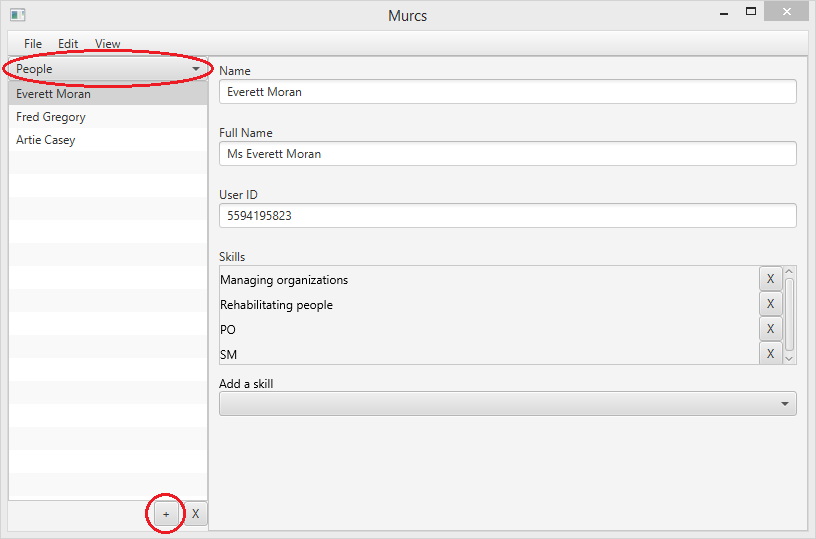
\includegraphics[width=\textwidth]{images/screenshots/people1.PNG}
\caption{Adding a Person Method 1}
\label{fig:new_project}
\end{figure}

The other method is to select File/New/Person from the File menu at the top of the application as shown in the fig below.

\begin{figure}[H]
\centering
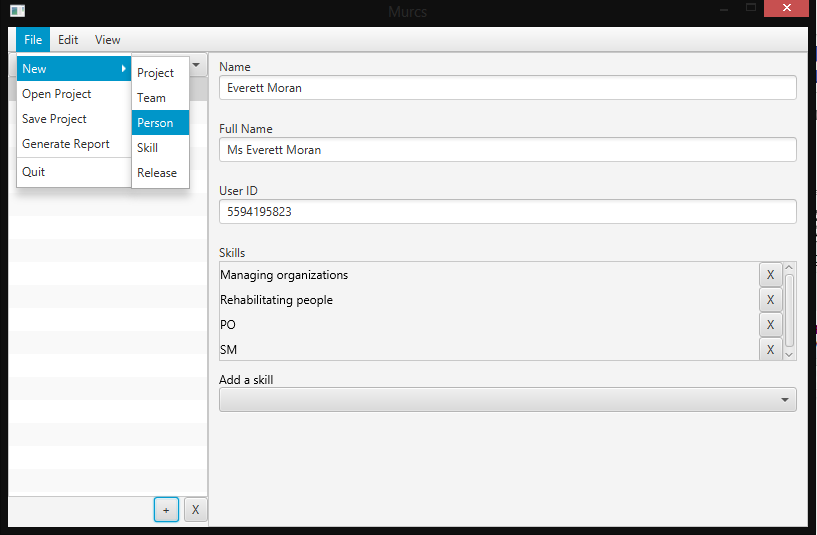
\includegraphics[width=\textwidth]{images/screenshots/people4.PNG}
\caption{Adding a Person Method 2}
\label{fig:new_project}
\end{figure}

Once you have clicked the add button or selected file/new/person a dialog will appear that asks for information about the new person you are creating. The minimum requirements for this are the Name and UserID, all of the other fields are optional. These fields include, a full name and a method for adding skills to the person.

\begin{figure}[H]
\centering
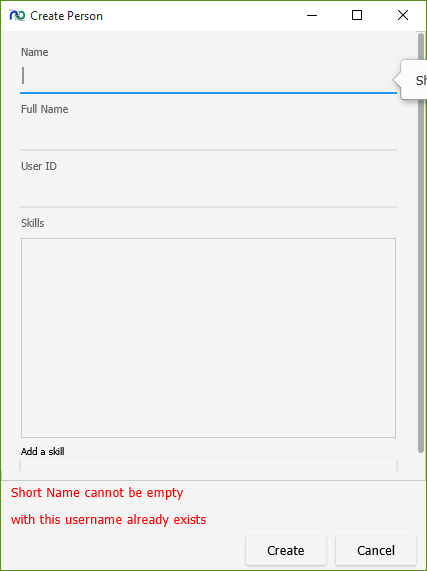
\includegraphics[width=\textwidth]{images/screenshots/people2.PNG}
\caption{Person Creation Dialog}
\label{fig:new_project}
\end{figure}

To add a skill simply select it from the drop down list (this is populated based on the skills you have added already) and it will appear in the list of skills. Then to remove a skill simply click x next to the skill. Note: If you add the PO skill to a person and then assign them to be PO of a Team and then remove the PO skill from them then they will be removed from the position of PO on that team.

\begin{figure}[H]
\centering
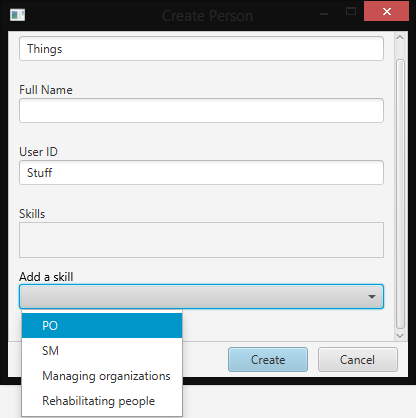
\includegraphics[width=\textwidth]{images/screenshots/people3.PNG}
\caption{Person adding/removing Skills}
\label{fig:new_project}
\end{figure}

In order to delete a person simply select it from the side list and click the X button next to the add button in the list display. When a person is deleted it will be removed from any place it is referenced in the application.

Once you have a person created you can add them to Teams which is covered in the Teams section of this user guide.